%% ============================================================
%% Reconfigurable DDR5 Memory Controller — MC Core
%% Technical Specification: Sub-Blocks, FSMs, Timing
%% Based on JESD79-5 (DDR5), DFI 5.2, AXI4
%% ============================================================
\documentclass[11pt,a4paper]{article}

%% ── Packages ─────────────────────────────────────────────────
\usepackage[a4paper,top=22mm,bottom=22mm,left=22mm,right=22mm]{geometry}
\usepackage[T1]{fontenc}
\usepackage[protrusion=false,expansion=false]{microtype}
\usepackage{booktabs}
\usepackage{longtable}
\usepackage{array}
\usepackage{tabularx}
\usepackage{multirow}
\usepackage{xcolor}
\usepackage{colortbl}
\usepackage{amsmath}
\usepackage{amssymb}
\usepackage{enumitem}
\usepackage{fancyhdr}
\usepackage{titlesec}
\usepackage{parskip}
\usepackage{mdframed}
\usepackage{hyperref}
\usepackage{tikz}
\usepackage{pgfplots}
\pgfplotsset{compat=1.18}
\usetikzlibrary{arrows.meta,positioning,shapes.geometric,fit,
                backgrounds,calc,decorations.pathreplacing,
                automata,shadows}

%% ── Colours ──────────────────────────────────────────────────
\definecolor{ddrblue}  {RGB}{25, 85,155}
\definecolor{ddrteal}  {RGB}{0, 120,110}
\definecolor{ddramber} {RGB}{190,120,  0}
\definecolor{ddrgreen} {RGB}{0, 125, 70}
\definecolor{ddrred}   {RGB}{170, 30, 30}
\definecolor{ddrpurple}{RGB}{100, 40,140}
\definecolor{lightgray}{RGB}{245,245,245}
\definecolor{midgray}  {RGB}{210,210,210}
\definecolor{rowblue}  {RGB}{232,242,255}
\definecolor{rowgreen} {RGB}{232,250,238}
\definecolor{roworange}{RGB}{255,244,225}
\definecolor{rowred}   {RGB}{255,236,236}
\definecolor{rowpurple}{RGB}{244,234,255}
\definecolor{rowteal}  {RGB}{228,248,246}
\definecolor{codebg}   {RGB}{250,250,252}

%% ── Hyperref ─────────────────────────────────────────────────
\hypersetup{colorlinks=true,linkcolor=ddrblue,urlcolor=ddrteal,
            pdftitle={RMC MC Core Technical Specification}}

%% ── Section style ────────────────────────────────────────────
\titleformat{\section}  {\large\bfseries\color{ddrblue}}{}{0em}{}[\titlerule]
\titleformat{\subsection}{\normalsize\bfseries\color{ddrteal}}{}{0em}{}
\titleformat{\subsubsection}{\normalsize\bfseries\color{ddramber}}{}{0em}{}

%% ── Header / Footer ──────────────────────────────────────────
\pagestyle{fancy}\fancyhf{}
\renewcommand{\headrulewidth}{0.4pt}
\fancyhead[L]{\small\textcolor{ddrblue}{\textbf{RMC — MC Core Specification}}}
\fancyhead[R]{\small\textcolor{gray}{JESD79-5 / DFI 5.2}}
\fancyfoot[C]{\small\thepage}

%% ── Column types ─────────────────────────────────────────────
\newcolumntype{L}[1]{>{\raggedright\arraybackslash}p{#1}}
\newcolumntype{C}[1]{>{\centering\arraybackslash}p{#1}}
\newcolumntype{R}[1]{>{\raggedleft\arraybackslash}p{#1}}

%% ── Macros ───────────────────────────────────────────────────
\newcommand{\sym}[1]{\texttt{\textbf{#1}}}
\newcommand{\reg}[1]{\textcolor{ddrpurple}{\texttt{#1}}}
\newcommand{\st}[1]{\textcolor{ddrblue}{\texttt{\textbf{#1}}}}
\newcommand{\trans}[1]{\textcolor{ddramber}{\textit{#1}}}

%% ── Framed boxes ─────────────────────────────────────────────
\newmdenv[backgroundcolor=rowblue,linecolor=ddrblue,linewidth=1pt,
  innerleftmargin=8pt,innerrightmargin=8pt,
  innertopmargin=6pt,innerbottommargin=6pt,roundcorner=4pt]{notebox}
\newmdenv[backgroundcolor=roworange,linecolor=ddramber,linewidth=1pt,
  innerleftmargin=8pt,innerrightmargin=8pt,
  innertopmargin=6pt,innerbottommargin=6pt,roundcorner=4pt]{warnbox}
\newmdenv[backgroundcolor=rowgreen,linecolor=ddrgreen,linewidth=1pt,
  innerleftmargin=8pt,innerrightmargin=8pt,
  innertopmargin=6pt,innerbottommargin=6pt,roundcorner=4pt]{specbox}

%% ── TikZ styles ──────────────────────────────────────────────
\tikzset{
  fsm/.style={draw=ddrblue,fill=rowblue,rounded corners=5pt,
              minimum width=2.4cm,minimum height=0.75cm,
              font=\small\bfseries,text=ddrblue,
              drop shadow={shadow xshift=0.5pt,shadow yshift=-0.5pt,
              opacity=0.2}},
  fsmred/.style={fsm,draw=ddrred,fill=rowred,text=ddrred},
  fsmgreen/.style={fsm,draw=ddrgreen,fill=rowgreen,text=ddrgreen},
  fsmamber/.style={fsm,draw=ddramber,fill=roworange,text=ddramber},
  fsmpurple/.style={fsm,draw=ddrpurple,fill=rowpurple,text=ddrpurple},
  arr/.style={-{Stealth[length=5pt,width=4pt]},thick,color=ddrteal},
  arrgray/.style={arr,color=gray},
  lbl/.style={font=\scriptsize,color=ddramber,fill=white,
              inner sep=1.5pt,rounded corners=2pt},
  blk/.style={draw=ddrblue,fill=rowblue,rounded corners=4pt,
              minimum width=2.8cm,minimum height=0.9cm,
              font=\small\bfseries,text=ddrblue},
  blkteal/.style={blk,draw=ddrteal,fill=rowteal,text=ddrteal},
  blkamber/.style={blk,draw=ddramber,fill=roworange,text=ddramber},
  blkred/.style={blk,draw=ddrred,fill=rowred,text=ddrred},
  blkpurple/.style={blk,draw=ddrpurple,fill=rowpurple,text=ddrpurple},
}

%% ─────────────────────────────────────────────────────────────
\begin{document}

% ── Title Page ───────────────────────────────────────────────
\begin{titlepage}\centering\vspace*{1.5cm}
{\Huge\bfseries\color{ddrblue}Reconfigurable DDR5 Memory Controller\\[0.5em]}
{\LARGE\color{ddrteal}MC Core — Technical Specification\\[0.4em]}
{\large Sub-Blocks $\cdot$ FSMs $\cdot$ Timing Constraints $\cdot$ DFI Interface}
\vspace{1.2cm}

\begin{center}
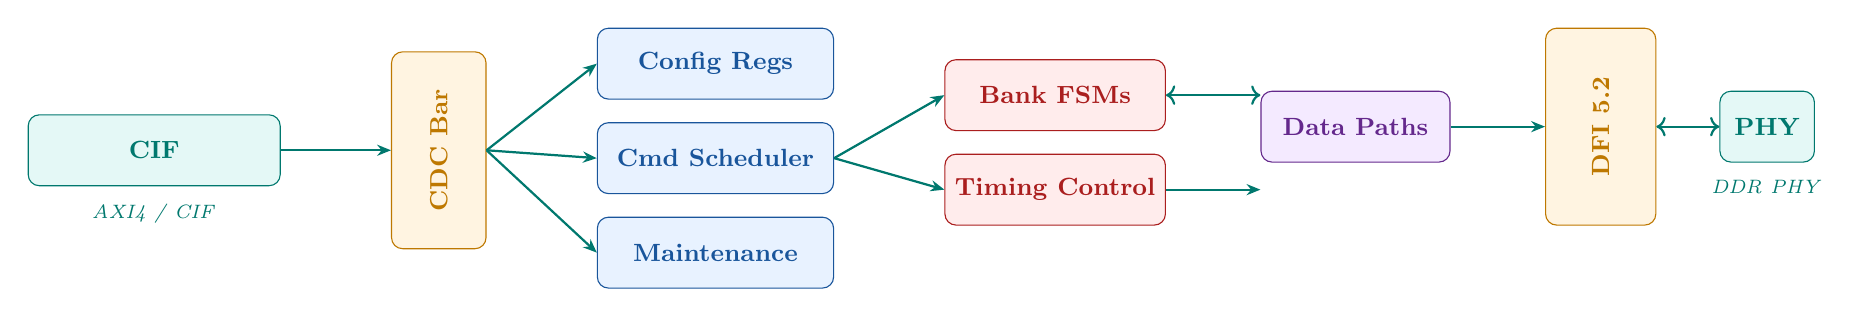
\begin{tikzpicture}[node distance=0.7cm and 1.2cm]
  % CIF
  \node[blkteal,minimum width=3.2cm](cif){CIF};
  % CDC
  \node[blkamber,right=1.4cm of cif,minimum width=1.2cm,minimum height=2.5cm](cdc){\rotatebox{90}{\small CDC Bar}};
  % MC Core blocks
  \node[blk,right=1.4cm of cdc,yshift=1.1cm,minimum width=3cm](cr){Config Regs};
  \node[blk,right=1.4cm of cdc,yshift=-0.1cm,minimum width=3cm](sched){Cmd Scheduler};
  \node[blk,right=1.4cm of cdc,yshift=-1.3cm,minimum width=3cm](maint){Maintenance};
  % DRAM Domain
  \node[blkred,right=1.4cm of sched,yshift=0.8cm,minimum width=2.8cm](bsm){Bank FSMs};
  \node[blkred,right=1.4cm of sched,yshift=-0.4cm,minimum width=2.8cm](tc){Timing Control};
  % Data paths
  \node[blkpurple,right=1.2cm of bsm,yshift=-0.4cm,minimum width=2.4cm](dp){Data Paths};
  % DFI
  \node[blkamber,right=1.2cm of dp,minimum width=1.4cm,minimum height=2.5cm](dfi){\rotatebox{90}{\small DFI 5.2}};
  % PHY
  \node[blkteal,right=0.8cm of dfi,minimum width=1.2cm](phy){PHY};

  % Arrows
  \draw[arr](cif.east)--(cdc.west);
  \draw[arr](cdc.east)--(cr.west);
  \draw[arr](cdc.east)--(sched.west);
  \draw[arr](cdc.east)--(maint.west);
  \draw[arr](sched.east)--(bsm.west);
  \draw[arr](sched.east)--(tc.west);
  \draw[arr,<->](bsm.east)--(dp.west|-bsm.east);
  \draw[arr](tc.east)--(dp.west|-tc.east);
  \draw[arr](dp.east)--(dfi.west);
  \draw[arr,<->](dfi.east)--(phy.west);

  % Labels
  \node[below=0.1cm of cif,font=\scriptsize,color=ddrteal]{\textit{AXI4 / CIF}};
  \node[below=0.1cm of phy,font=\scriptsize,color=ddrteal]{\textit{DDR PHY}};
\end{tikzpicture}
\end{center}

\vspace{0.8cm}
\begin{tabular}{ll}
\textbf{Standard}   & JEDEC JESD79-5 (DDR5), DFI 5.2, AXI4 \\
\textbf{Banks}      & 16 (2 BG $\times$ 4 banks $\times$ 2 sub-channels) \\
\textbf{Burst}      & BL16 (BL/2 = 8 clock cycles) \\
\textbf{Clock}      & Dual domain: AXI (CIF) / MC (DRAM) \\
\textbf{Total FSMs} & $\approx$23 (1 Init + 16 BSM + 6 Maintenance/Scheduler) \\
\end{tabular}
\vfill
{\small\color{gray}Memory Controller Capstone Project --- Based on JESD79-5}
\end{titlepage}

\tableofcontents\newpage

%% ════════════════════════════════════════════════════════════
\section{Overview and Architecture}

The MC Core sits between the Client Interface (CIF) clock domain and the DRAM
domain, connected via a single Async FIFO CDC bar. It is responsible for all
DRAM command scheduling, timing enforcement, refresh management, power state
control, and initialisation sequencing.

\subsection{Clock Domains}

\begin{center}
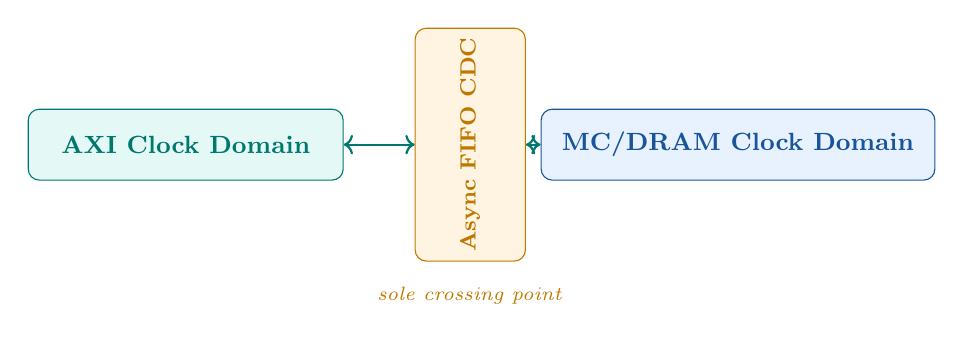
\begin{tikzpicture}[node distance=0.5cm and 1.5cm]
  \node[blkteal,minimum width=4cm](axi){AXI Clock Domain};
  \node[blk,right=2.5cm of axi,minimum width=5cm](mc){MC/DRAM Clock Domain};
  \node[blkamber,minimum width=1.4cm,minimum height=1.5cm,
        right=1.2cm of axi,xshift=-0.3cm](cdc){\rotatebox{90}{\footnotesize Async FIFO CDC}};
  \draw[arr,<->](axi.east)--(cdc.west);
  \draw[arr,<->](cdc.east)--(mc.west);
  \node[below=0.2cm of cdc,font=\scriptsize,color=ddramber]{\textit{sole crossing point}};
\end{tikzpicture}
\end{center}

\subsection{Sub-Block Inventory}

\begin{longtable}{L{3.2cm} L{2cm} L{9.3cm}}
\toprule
\textbf{Sub-Block} & \textbf{Domain} & \textbf{Function} \\
\midrule
\endfirsthead\toprule\textbf{Sub-Block}&\textbf{Domain}&\textbf{Function}\\\midrule\endhead\bottomrule\endfoot
\rowcolor{rowblue}
Config Registers     & MC & Holds all timing parameters (tRCD, tRAS, tRP, tRFC, tREFI, CL, CWL, BL, \ldots), refresh mode, page policy, RFM thresholds. Written via AXI4-Lite CSR path. \\
Init FSM             & MC & Full DDR5 power-up and reset sequence per JESD79-5 §3.3.1/3.3.2. Issues RESET\_n, NOP burst, DLL reset, ZQcal, MRW sequence. Single instance. \\
\rowcolor{rowblue}
Bank State Machines  & MC & One FSM per bank (16 total). Tracks state (Idle/Active/Reading/Writing/Precharging/Refreshing/SR/PD) and per-bank timers. \\
Timing Control       & MC & Per-bank timer array + cross-bank constraint checker. Computes \texttt{cmd\_ok[bank][cmd\_type]} every cycle fed to Scheduler. \\
\rowcolor{rowblue}
DDR Cmd Scheduler    & MC & Arbitrates between read/write pools, issues final DFI command. Enforces page policy (open/closed/adaptive). \\
Refresh Scheduler    & MC & Tracks tREFI budget (leaky bucket), decides REFab vs REFsb, handles postponement up to $8\times$tREFI. \\
\rowcolor{rowblue}
ZQcal FSM            & MC & Periodic impedance calibration via MPC ZQCAL Start/Latch sequence. \\
RFM FSM              & MC & DDR5 rowhammer mitigation. Per-bank RAA counter; triggers RFM command when RAA $\leq$ RAAIMT. \\
\rowcolor{rowblue}
Power Management FSM & MC & CKE-controlled transitions: Active PD, Precharge PD, Self-Refresh, MPSM. \\
Write Data Path      & MC & Write data buffer, DM/ECC generator, Write CRC computation, DFI write timing insertion. \\
\rowcolor{rowblue}
Read Data Path       & MC & Read data capture FIFO, Read CRC/ECC checker, Read latency counter, ECS FSM. \\
\end{longtable}

%% ════════════════════════════════════════════════════════════
\section{Config Registers}

All timing knobs consumed by the MC Core are held here, programmed by the host
before init kick and updatable (with care) at runtime.

\begin{longtable}{L{3cm} L{2cm} L{9.3cm}}
\toprule
\textbf{Register} & \textbf{Width} & \textbf{Description} \\
\midrule
\endfirsthead\toprule\textbf{Register}&\textbf{Width}&\textbf{Description}\\\midrule\endhead\bottomrule\endfoot
\rowcolor{rowblue}
\reg{CL}          & 7b & CAS Latency (nCK) \\
\reg{CWL}         & 7b & CAS Write Latency = CL$-$2 (nCK) \\
\rowcolor{rowblue}
\reg{tRCD}        & 8b & RAS-to-CAS delay (nCK) \\
\reg{tRP}         & 8b & Row Precharge Time (nCK) \\
\rowcolor{rowblue}
\reg{tRAS}        & 9b & Row Active Time min (nCK) \\
\reg{tRC}         & 9b & Row Cycle Time = tRAS+tRP (nCK) \\
\rowcolor{rowblue}
\reg{tWR}         & 8b & Write Recovery Time (nCK) \\
\reg{tRTP}        & 6b & Internal Read-to-Precharge (nCK) \\
\rowcolor{rowblue}
\reg{tCCD\_L}     & 5b & CAS-to-CAS same BG (nCK) \\
\reg{tCCD\_S}     & 5b & CAS-to-CAS diff BG = BL/2 (nCK) \\
\rowcolor{rowblue}
\reg{tWTR\_L}     & 6b & Write-to-Read same BG (nCK) \\
\reg{tWTR\_S}     & 5b & Write-to-Read diff BG (nCK) \\
\rowcolor{rowblue}
\reg{tRRD\_L}     & 5b & ACT-to-ACT same BG (nCK) \\
\reg{tRRD\_S}     & 4b & ACT-to-ACT diff BG (nCK) \\
\rowcolor{rowblue}
\reg{tFAW}        & 6b & Four-Activate Window (nCK) \\
\reg{tRFC1}       & 12b & Refresh Cycle Time 1x (nCK) \\
\rowcolor{rowblue}
\reg{tRFCsb}      & 11b & Same-Bank RFC (nCK) \\
\reg{tREFI}       & 14b & Average Refresh Interval (nCK) \\
\rowcolor{rowblue}
\reg{tMRD}        & 5b & MRS-to-MRS (nCK) \\
\reg{tXP}         & 5b & PDX-to-Command (nCK) \\
\rowcolor{rowblue}
\reg{tXS}         & 12b & SRX-to-Command no DLL (nCK) \\
\reg{tCKSRE}      & 5b & Clock stable after SRE (nCK) \\
\rowcolor{rowblue}
\reg{tCKSRX}      & 5b & Clock stable before SRX (nCK) \\
\reg{tDLLK}       & 11b & DLL Lock Time (nCK) \\
\rowcolor{rowblue}
\reg{RAAIMT}      & 8b & RFM RAA Initial Management Threshold \\
\reg{RAAMMT}      & 8b & RFM RAA Maximum Management Threshold \\
\rowcolor{rowblue}
\reg{RAADec}      & 4b & RAA decrement per REF command \\
\reg{REF\_MODE}   & 2b & 00=REFab, 01=REFsb, 10=FGR-2x, 11=FGR-4x \\
\rowcolor{rowblue}
\reg{PAGE\_POLICY}& 2b & 00=Open, 01=Closed, 10=Adaptive \\
\reg{INIT\_KICK}  & 1b & Write 1 to start Init FSM \\
\rowcolor{rowblue}
\reg{SOFT\_RESET} & 1b & Synchronous soft-reset all FSMs \\
\end{longtable}

%% ════════════════════════════════════════════════════════════
\section{Init FSM}

\begin{notebox}
\textbf{Reference:} JESD79-5 §3.3.1 (power-up with stable power) and §3.3.2 (reset with stable power).
Single instance. Triggered by \reg{INIT\_KICK}. Releases \texttt{init\_done} to the Cmd Scheduler.
\end{notebox}

\subsection{State Diagram}

\begin{center}
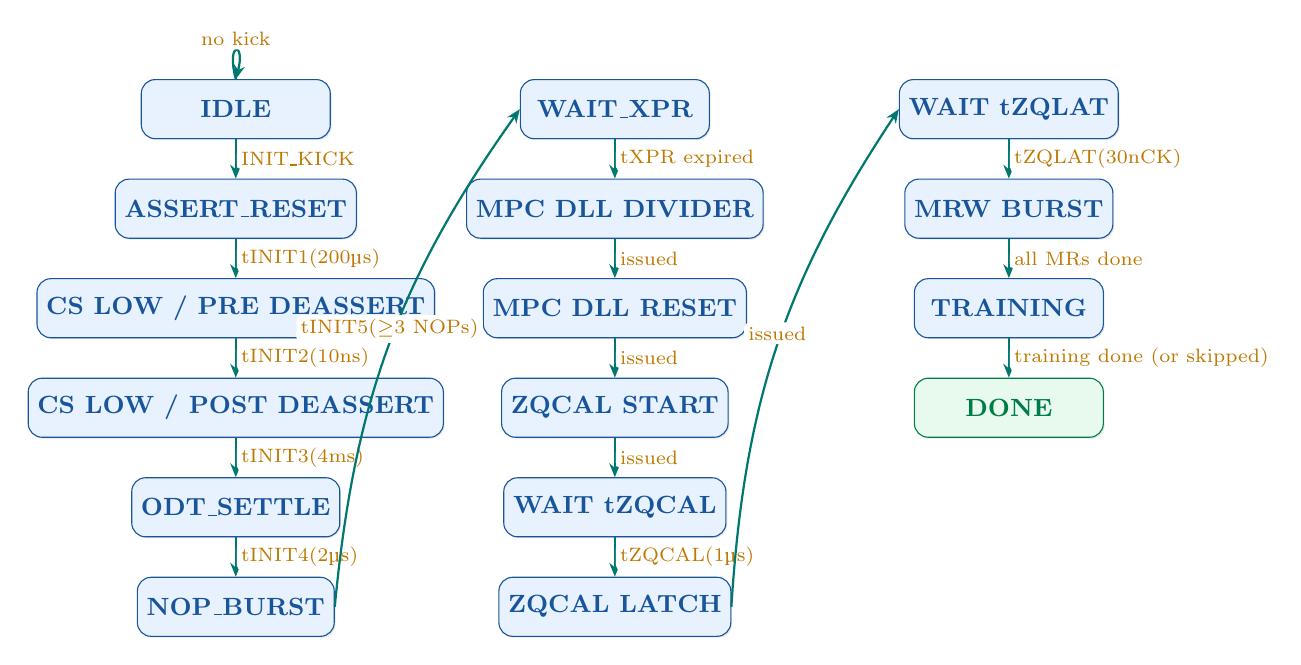
\begin{tikzpicture}[node distance=0.5cm and 0.4cm,>=Stealth]
  % Column 1
  \node[fsm](IDLE)                          {IDLE};
  \node[fsm,below=of IDLE](RST_LOW)         {ASSERT\_RESET};
  \node[fsm,below=of RST_LOW](CS_PRE_RST)   {CS LOW / PRE DEASSERT};
  \node[fsm,below=of CS_PRE_RST](CS_POST)   {CS LOW / POST DEASSERT};
  \node[fsm,below=of CS_POST](ODT_SETTLE)   {ODT\_SETTLE};
  \node[fsm,below=of ODT_SETTLE](NOP_BURST) {NOP\_BURST};
  % Column 2
  \node[fsm,right=2.4cm of IDLE](WAIT_XPR) {WAIT\_XPR};
  \node[fsm,below=of WAIT_XPR](DLL_DIV)    {MPC DLL DIVIDER};
  \node[fsm,below=of DLL_DIV](DLL_RST)     {MPC DLL RESET};
  \node[fsm,below=of DLL_RST](ZQCAL_START) {ZQCAL START};
  \node[fsm,below=of ZQCAL_START](WAIT_ZQ) {WAIT tZQCAL};
  \node[fsm,below=of WAIT_ZQ](ZQCAL_LATCH) {ZQCAL LATCH};
  % Column 3
  \node[fsm,right=2.4cm of WAIT_XPR](WAIT_ZLAT) {WAIT tZQLAT};
  \node[fsm,below=of WAIT_ZLAT](MRW_BURST)      {MRW BURST};
  \node[fsm,below=of MRW_BURST](TRAIN_DISPATCH)  {TRAINING};
  \node[fsmgreen,below=of TRAIN_DISPATCH](DONE)  {DONE};

  % Arrows col1 down
  \draw[arr](IDLE)       -- node[lbl,right]{INIT\_KICK} (RST_LOW);
  \draw[arr](RST_LOW)    -- node[lbl,right]{tINIT1(200µs)} (CS_PRE_RST);
  \draw[arr](CS_PRE_RST) -- node[lbl,right]{tINIT2(10ns)} (CS_POST);
  \draw[arr](CS_POST)    -- node[lbl,right]{tINIT3(4ms)} (ODT_SETTLE);
  \draw[arr](ODT_SETTLE) -- node[lbl,right]{tINIT4(2µs)} (NOP_BURST);
  \draw[arr](NOP_BURST.east) to[bend left=15] node[lbl,above]{tINIT5($\geq$3 NOPs)} (WAIT_XPR.west);

  % Arrows col2 down
  \draw[arr](WAIT_XPR)    -- node[lbl,right]{tXPR expired} (DLL_DIV);
  \draw[arr](DLL_DIV)     -- node[lbl,right]{issued} (DLL_RST);
  \draw[arr](DLL_RST)     -- node[lbl,right]{issued} (ZQCAL_START);
  \draw[arr](ZQCAL_START) -- node[lbl,right]{issued} (WAIT_ZQ);
  \draw[arr](WAIT_ZQ)     -- node[lbl,right]{tZQCAL(1µs)} (ZQCAL_LATCH);
  \draw[arr](ZQCAL_LATCH.east) to[bend left=15] node[lbl,above]{issued} (WAIT_ZLAT.west);

  % Arrows col3 down
  \draw[arr](WAIT_ZLAT)      -- node[lbl,right]{tZQLAT(30nCK)} (MRW_BURST);
  \draw[arr](MRW_BURST)      -- node[lbl,right]{all MRs done} (TRAIN_DISPATCH);
  \draw[arr](TRAIN_DISPATCH) -- node[lbl,right]{training done (or skipped)} (DONE);

  % Self-loop on IDLE
  \draw[arr](IDLE.north) to[loop above] node[lbl]{no kick} (IDLE.north);
\end{tikzpicture}
\end{center}

\subsection{State Descriptions}

\begin{longtable}{L{3.2cm} L{11.3cm}}
\toprule
\textbf{State} & \textbf{Action / Exit Condition} \\
\midrule
\endfirsthead\toprule\textbf{State}&\textbf{Action / Exit}\\\midrule\endhead\bottomrule\endfoot
\rowcolor{rowblue}
\st{IDLE}            & Wait for \reg{INIT\_KICK}=1. Assert RESET\_n=0, CKE=0, CS\_n=0. \\
\st{ASSERT\_RESET}   & Hold RESET\_n LOW. Count 200\,µs (tINIT1). CS\_n held LOW. Exit when timer expires. \\
\rowcolor{rowblue}
\st{CS\_LOW\_PRE\_DEASSERT} & Hold CS\_n LOW for $\geq$tINIT2=10\,ns before deasserting RESET\_n. \\
\st{CS\_LOW\_POST\_DEASSERT} & Deassert RESET\_n (HIGH). CS\_n remains LOW for tINIT3=4\,ms. CKE still LOW. \\
\rowcolor{rowblue}
\st{ODT\_SETTLE}     & Raise CKE (stable CK already running). Wait tINIT4=2\,µs for ODT and CK settle. \\
\st{NOP\_BURST}      & Issue $\geq$3 NOP/DES commands (tINIT5). CS\_n now driven normally. \\
\rowcolor{rowblue}
\st{WAIT\_XPR}       & Wait tXPR = max(5nCK, tRFC1+10\,ns) after CS\_n first high. \\
\st{MPC\_DLL\_DIVIDER} & Issue MPC: DLL Divider Select (configures tCCD\_L divider via MR13). \\
\rowcolor{rowblue}
\st{MPC\_DLL\_RESET} & Issue MPC: DLL Reset. Required before ZQcal per spec. \\
\st{ZQCAL\_START}    & Issue MPC: ZQCAL Start. Starts impedance calibration. \\
\rowcolor{rowblue}
\st{WAIT\_tZQCAL}    & Count tZQCAL=1\,µs. \\
\st{ZQCAL\_LATCH}    & Issue MPC: ZQCAL Latch. Latches calibrated driver/ODT codes. \\
\rowcolor{rowblue}
\st{WAIT\_tZQLAT}    & Count tZQLAT=30\,nCK. \\
\st{MRW\_BURST}      & Issue MRW to all required mode registers (MR0, MR2, MR4, MR5, MR6, MR8, MR13, \ldots). One MRW per tMRD (16\,nCK). \\
\rowcolor{rowblue}
\st{TRAINING\_DISPATCH} & Optional: CA training, CS training, Write Levelling, Read training. Controlled by \reg{TRAIN\_EN} bits. \\
\st{DONE}            & Assert \texttt{init\_done}. Release Cmd Scheduler from reset. \\
\end{longtable}

%% ════════════════════════════════════════════════════════════
\section{Bank State Machines (BSM)}

\begin{notebox}
16 instances (one per bank). Each BSM receives commands from the Cmd Scheduler
and \texttt{cmd\_ok} enable from Timing Control. All bank-private timers live here.
\end{notebox}

\subsection{State Diagram (single bank)}

\begin{center}
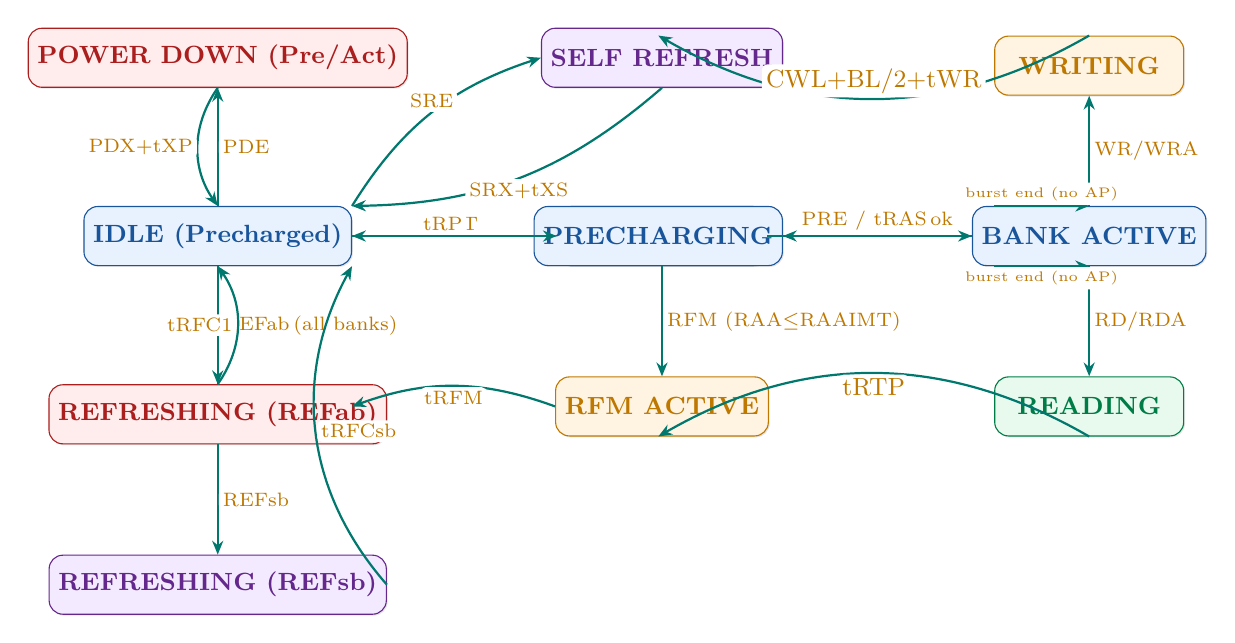
\begin{tikzpicture}[node distance=0.8cm and 2.2cm,>=Stealth]
  \node[fsm]          (IDLE)  {IDLE (Precharged)};
  \node[fsm,right=2.6cm of IDLE] (ACT)   {ACTIVATING};
  \node[fsm,right=2.6cm of ACT]  (ACTIVE){BANK ACTIVE};

  \node[fsmgreen,below=1.4cm of ACTIVE](RD)  {READING};
  \node[fsmamber,above=1.4cm of ACTIVE](WR)  {WRITING};

  \node[fsm,left=2.4cm of ACTIVE](PRE) {PRECHARGING};

  \node[fsmred,below=1.5cm of IDLE](REF)   {REFRESHING (REFab)};
  \node[fsmpurple,below=1.4cm of REF](SB)  {REFRESHING (REFsb)};

  \node[fsmred,above=1.5cm of IDLE](PD)    {POWER DOWN (Pre/Act)};
  \node[fsmpurple,above=1.5cm of ACT](SR)  {SELF REFRESH};
  \node[fsmamber,below=1.4cm of ACT](RFM)  {RFM ACTIVE};

  % Main row
  \draw[arr](IDLE)  -- node[lbl,above]{ACT}     (ACT);
  \draw[arr](ACT)   -- node[lbl,above]{tRCD}    (ACTIVE);

  % Active to Read/Write
  \draw[arr](ACTIVE) -- node[lbl,right]{RD/RDA}  (RD);
  \draw[arr](ACTIVE) -- node[lbl,right]{WR/WRA}  (WR);

  % Read/Write back to Active
  \draw[arr](RD.west|-ACTIVE.south) -- node[lbl,below]{\tiny burst end (no AP)} (ACTIVE.south);
  \draw[arr](WR.west|-ACTIVE.north) -- node[lbl,above]{\tiny burst end (no AP)} (ACTIVE.north);

  % Active / RD / WR to PRE
  \draw[arr](ACTIVE.west) -- node[lbl,above]{PRE / tRAS\,ok} (PRE.east);
  \draw[arr](RD.south)    to[bend right=30] node[lbl,below]{\small tRTP} (PRE.south|-RD.south);
  \draw[arr](WR.north)    to[bend left=30]  node[lbl,above]{\small CWL+BL/2+tWR} (PRE.north|-WR.north);

  % PRE to IDLE
  \draw[arr](PRE.west) -- node[lbl,above]{tRP} (IDLE.east);

  % IDLE to REF
  \draw[arr](IDLE.south) -- node[lbl,right]{REFab\,(all banks)} (REF.north);
  \draw[arr](REF.north)  to[bend right=35] node[lbl,left]{tRFC1} (IDLE.south);

  % IDLE to REFsb
  \draw[arr](IDLE.south|-REF.south) -- node[lbl,right]{REFsb} (SB.north);
  \draw[arr](SB.east) to[bend left=35] node[lbl,right]{tRFCsb} (IDLE.south east);

  % IDLE to PD
  \draw[arr](IDLE.north) -- node[lbl,right]{PDE} (PD.south);
  \draw[arr](PD.south)   to[bend right=35] node[lbl,left]{PDX+tXP} (IDLE.north);

  % IDLE to SR
  \draw[arr](IDLE.north east) to[bend left=20] node[lbl,above]{SRE} (SR.west);
  \draw[arr](SR.south)        to[bend left=20] node[lbl,below]{SRX+tXS} (IDLE.north east);

  % IDLE to RFM
  \draw[arr](ACT.south) -- node[lbl,right]{RFM (RAA$\leq$RAAIMT)} (RFM.north);
  \draw[arr](RFM.west)  to[bend right=20] node[lbl,below]{tRFM} (IDLE.east|-RFM.west);
\end{tikzpicture}
\end{center}

\subsection{Bank State Descriptions}

\begin{longtable}{L{2.8cm} L{4.5cm} L{7.2cm}}
\toprule
\textbf{State} & \textbf{Legal Input Commands} & \textbf{Timer / Exit Condition} \\
\midrule
\endfirsthead\toprule\textbf{State}&\textbf{Legal Inputs}&\textbf{Timer/Exit}\\\midrule\endhead\bottomrule\endfoot
\rowcolor{rowblue}
\st{IDLE}      & ACT, REFab, REFsb, PDE, SRE, RFM & No timer. Exit on received command. \\
\st{ACTIVATING}& (none, internal) & tRCD counter. Transition to ACTIVE when expired. \\
\rowcolor{rowblue}
\st{BANK ACTIVE}& RD, RDA, WR, WRA, PRE, PREA & tRAS timer ensures minimum row open time. PRE only after tRAS satisfied. \\
\st{READING}   & BST (early termination) & CL + BL/2 until burst end. If RDA: AP started internally at tRTP. \\
\rowcolor{rowblue}
\st{WRITING}   & BST (early termination) & CWL + BL/2 until burst end. If WRA: AP started at CWL+BL/2. \\
\st{PRECHARGING}& (none) & tRP counter. Transition to IDLE when expired. \\
\rowcolor{rowblue}
\st{REFRESHING (REFab)} & (none) & tRFC1 counter. All 16 banks forced into this state simultaneously. \\
\st{REFRESHING (REFsb)} & (none) & tRFCsb counter. Only target bank locked; others remain accessible. \\
\rowcolor{rowblue}
\st{POWER DOWN} & PDX & Precharge PD (from IDLE) or Active PD (from ACTIVE). tCKE minimum low time. \\
\st{SELF REFRESH}& SRX & tCKSRE after entry; tCKESR minimum SR time; SRX raises CKE; tXS before commands. \\
\rowcolor{rowblue}
\st{RFM ACTIVE} & (none) & tRFM counter. Issued by Maintenance Engine when RAA $\leq$ RAAIMT. \\
\end{longtable}

\subsection{Per-Bank Timer Summary}

\begin{center}
\begin{tabular}{L{3.5cm} L{5cm} L{5.5cm}}
\toprule
\textbf{Timer} & \textbf{Loaded By} & \textbf{Condition Checked Before} \\
\midrule
\rowcolor{rowblue}
tRCD counter    & ACT issued          & Enabling RD/WR on same bank \\
tRAS counter    & ACT issued          & Enabling PRE/PREA on same bank \\
\rowcolor{rowblue}
tRC counter     & ACT issued          & Enabling next ACT on same bank \\
tRP counter     & PRE issued          & Enabling ACT on same bank \\
\rowcolor{rowblue}
tWR counter     & WR burst end        & Enabling PRE on same bank \\
tRTP counter    & RD burst start      & Enabling PRE on same bank \\
\rowcolor{rowblue}
tRFC1 counter   & REFab issued        & Enabling any cmd after refresh \\
tRFCsb counter  & REFsb issued        & Enabling cmd on refreshed bank \\
\rowcolor{rowblue}
tXS counter     & SRX asserted        & Enabling ACT after self-refresh exit \\
tXP counter     & PDX asserted        & Enabling cmd after power-down exit \\
\rowcolor{rowblue}
tMRD counter    & MRW issued          & Enabling next MRW \\
\bottomrule
\end{tabular}
\end{center}

%% ════════════════════════════════════════════════════════════
\section{Timing Control}

The Timing Control block is not an FSM — it is a \textit{combinational + registered
timer array} that outputs \texttt{cmd\_ok[15:0][CMD\_TYPES]} every cycle.

\subsection{Cross-Bank Constraints}

\begin{longtable}{L{3.2cm} L{3.2cm} L{8.1cm}}
\toprule
\textbf{Constraint} & \textbf{Scope} & \textbf{Implementation} \\
\midrule
\endfirsthead\toprule\textbf{Constraint}&\textbf{Scope}&\textbf{Implementation}\\\midrule\endhead\bottomrule\endfoot
\rowcolor{rowblue}
tRRD\_L  & Same BG, any bank    & Timestamp of last ACT in same BG; check $T_{\text{now}} - T_{\text{last\_ACT\_BG}} \geq$ tRRD\_L \\
tRRD\_S  & Diff BG, any bank    & Timestamp of last ACT globally; check $T_{\text{now}} - T_{\text{last\_ACT\_any}} \geq$ tRRD\_S \\
\rowcolor{rowblue}
tFAW     & All banks            & Sliding window: ring buffer of 4 most recent ACT timestamps. Block new ACT if oldest is within tFAW. \\
tCCD\_L  & Same BG, RD$\to$RD or WR$\to$WR & Timestamp of last RD/WR in same BG; enforce $\geq$ tCCD\_L \\
\rowcolor{rowblue}
tCCD\_S  & Diff BG              & Timestamp of last RD/WR globally; enforce $\geq$ tCCD\_S \\
tWTR\_L  & Same BG, WR$\to$RD  & Timestamp of last write data end in same BG; enforce $\geq$ WL+BL/2+tWTR\_L \\
\rowcolor{rowblue}
tWTR\_S  & Diff BG, WR$\to$RD  & Same but tWTR\_S window; enforce $\geq$ WL+BL/2+tWTR\_S \\
tRTW     & Any, RD$\to$WR       & Timestamp of last RD; enforce $\geq$ RL+BL/2$-$WL+2+tWPRE \\
\bottomrule
\end{longtable}

%% ════════════════════════════════════════════════════════════
\section{DDR Command Scheduler}

\begin{notebox}
The Scheduler is the arbitration heart of the MC Core. It consumes \texttt{cmd\_ok}
from Timing Control, bank states from BSMs, and pending transactions from the Read/Write
Cmd Pools. It issues one DFI command per clock cycle.
\end{notebox}

\subsection{Scheduler FSM}

\begin{center}
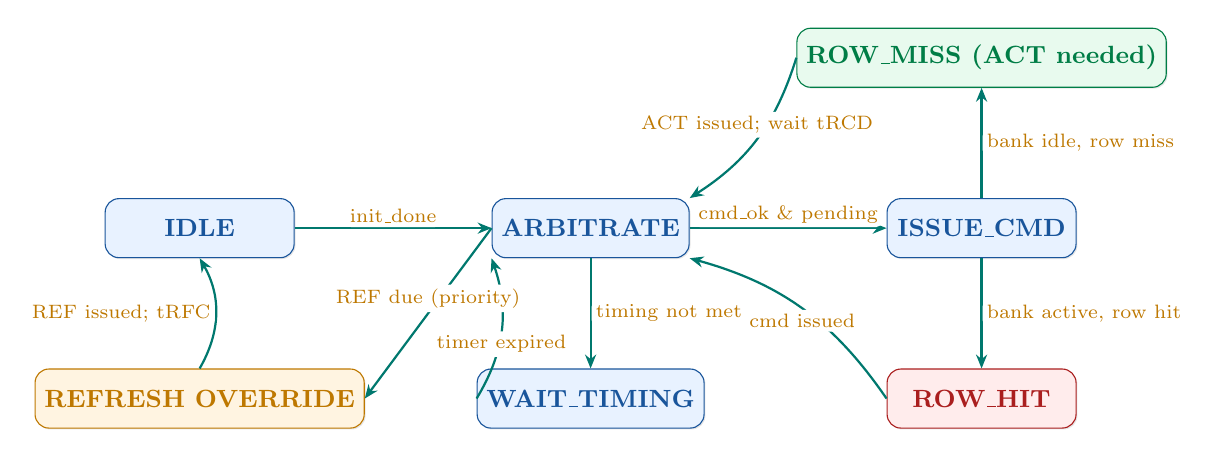
\begin{tikzpicture}[node distance=0.9cm and 2.2cm,>=Stealth]
  \node[fsm](IDLE2)     {IDLE};
  \node[fsm,right=2.5cm of IDLE2](ARB)    {ARBITRATE};
  \node[fsm,right=2.5cm of ARB](ISSUE)    {ISSUE\_CMD};
  \node[fsm,below=1.4cm of ARB](WAIT)     {WAIT\_TIMING};
  \node[fsmred,below=1.4cm of ISSUE](RHIT) {ROW\_HIT};
  \node[fsmgreen,above=1.4cm of ISSUE](RMISS){ROW\_MISS (ACT needed)};
  \node[fsmamber,below=1.4cm of IDLE2](REF2){REFRESH OVERRIDE};

  \draw[arr](IDLE2) -- node[lbl,above]{init\_done} (ARB);
  \draw[arr](ARB)   -- node[lbl,above]{cmd\_ok \& pending} (ISSUE);
  \draw[arr](ARB.south) -- node[lbl,right]{timing not met} (WAIT.north);
  \draw[arr](WAIT.west) to[bend right=25] node[lbl,below]{timer expired} (ARB.south west);
  \draw[arr](ISSUE) -- node[lbl,right]{bank active, row hit} (RHIT);
  \draw[arr](ISSUE) -- node[lbl,right]{bank idle, row miss} (RMISS);
  \draw[arr](RHIT.west) to[bend right=20] node[lbl,below]{cmd issued} (ARB.south east);
  \draw[arr](RMISS.west) to[bend left=20] node[lbl,above]{ACT issued; wait tRCD} (ARB.north east);
  \draw[arr](ARB.west) -- node[lbl,above]{REF due (priority)} (REF2.east);
  \draw[arr](REF2.north) to[bend right=30] node[lbl,left]{REF issued; tRFC} (IDLE2.south);
\end{tikzpicture}
\end{center}

\subsection{Page Policy}

\begin{longtable}{L{3cm} L{11.5cm}}
\toprule
\textbf{Policy} & \textbf{Behaviour} \\
\midrule
\endfirsthead\toprule\textbf{Policy}&\textbf{Behaviour}\\\midrule\endhead\bottomrule\endfoot
\rowcolor{rowblue}
Open Page   & Row stays open after RD/WR. Next access to same row = row hit (no ACT needed). Best for sequential/localised access. \\
Closed Page & Auto-precharge every RD/WR (RDA/WRA). Row is always idle. Best for random access patterns. \\
\rowcolor{rowblue}
Adaptive    & Track hit/miss ratio per bank. Switch to closed-page if miss rate exceeds threshold (configurable in \reg{PAGE\_POLICY\_THRESH}). \\
\end{longtable}

\subsection{Command Priority Order}

{\small
\begin{enumerate}[leftmargin=1.5em,itemsep=2pt]
  \item \textbf{Refresh Override} (REF budget about to expire — highest priority)
  \item \textbf{RFM} (RAA $\leq$ RAAIMT — safety critical)
  \item \textbf{ZQcal} (periodic, low urgency until overdue)
  \item \textbf{Write drain} (if write buffer nearly full)
  \item \textbf{Row-hit reads} (open page, same row)
  \item \textbf{Row-hit writes}
  \item \textbf{Row-miss reads} (ACT $\to$ wait tRCD $\to$ RD)
  \item \textbf{Row-miss writes}
  \item \textbf{PRE} (close idle banks if closed-page policy)
\end{enumerate}
}

%% ════════════════════════════════════════════════════════════
\section{Maintenance Engine}

The Maintenance Engine houses four sub-FSMs that handle all autonomous background
operations. Each sub-FSM runs independently and posts requests to the Scheduler via
a priority request bus.

\subsection{6a — Refresh Scheduler FSM}

\begin{center}
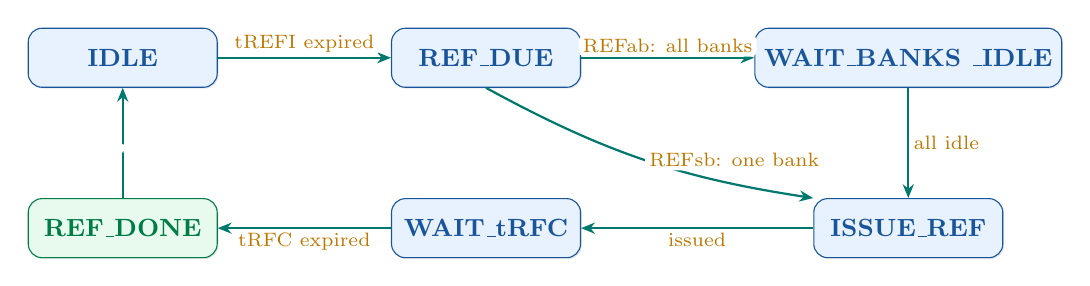
\begin{tikzpicture}[node distance=0.9cm and 2.2cm,>=Stealth]
  \node[fsm](RI)    {IDLE};
  \node[fsm,right=2.2cm of RI](RD2)  {REF\_DUE};
  \node[fsm,right=2.2cm of RD2](RW)  {WAIT\_BANKS \_IDLE};
  \node[fsm,below=1.4cm of RW](RIS)  {ISSUE\_REF};
  \node[fsm,below=1.4cm of RD2](RWT) {WAIT\_tRFC};
  \node[fsmgreen,below=1.4cm of RI](RDONE){REF\_DONE};

  \draw[arr](RI)  -- node[lbl,above]{tREFI expired} (RD2);
  \draw[arr](RD2) -- node[lbl,above]{REFab: all banks} (RW);
  \draw[arr](RD2.south) to[bend right=10] node[lbl,right]{REFsb: one bank} (RIS.north west);
  \draw[arr](RW)  -- node[lbl,right]{all idle} (RIS);
  \draw[arr](RIS) -- node[lbl,below]{issued} (RWT);
  \draw[arr](RWT) -- node[lbl,below]{tRFC expired} (RDONE);
  \draw[arr](RDONE) -- node[lbl,below]{} (RI);
\end{tikzpicture}
\end{center}

\textbf{Leaky-bucket logic:} A counter increments by 1 every tREFI. If it reaches 9 (max postponement = $8\times$tREFI), the Refresh FSM asserts highest-priority override to the Scheduler. Decrement by 1 on each REF issued.

\textbf{FGR (Fine Granularity):} When \reg{REF\_MODE}[1:0] = 10 or 11, tRFC is replaced by tRFC2 or tRFC4 from Config Regs, and the budget counter threshold is halved or quartered accordingly.

\subsection{6b — ZQcal FSM}

\begin{center}
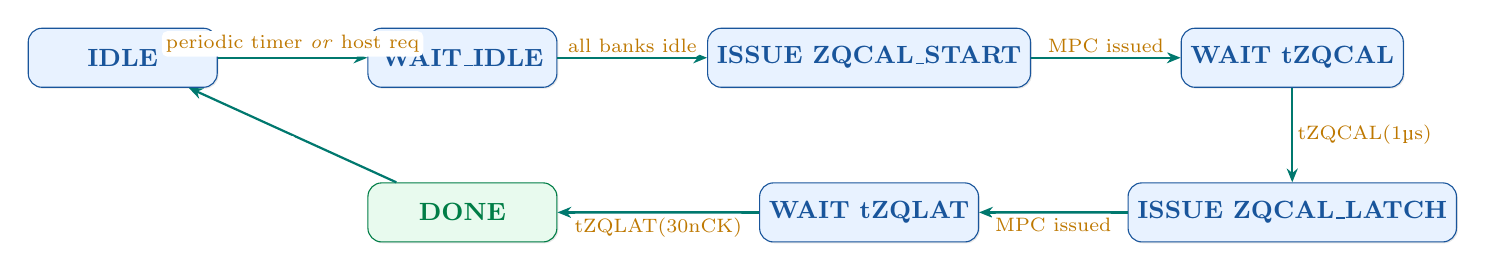
\begin{tikzpicture}[node distance=0.7cm and 2cm,>=Stealth]
  \node[fsm](ZI)   {IDLE};
  \node[fsm,right=1.9cm of ZI](ZW)   {WAIT\_IDLE};
  \node[fsm,right=1.9cm of ZW](ZS)   {ISSUE ZQCAL\_START};
  \node[fsm,right=1.9cm of ZS](ZT)   {WAIT tZQCAL};
  \node[fsm,below=1.2cm of ZT](ZL)   {ISSUE ZQCAL\_LATCH};
  \node[fsm,below=1.2cm of ZS](ZLW)  {WAIT tZQLAT};
  \node[fsmgreen,below=1.2cm of ZW](ZD){DONE};

  \draw[arr](ZI) -- node[lbl,above]{periodic timer \textit{or} host req} (ZW);
  \draw[arr](ZW) -- node[lbl,above]{all banks idle} (ZS);
  \draw[arr](ZS) -- node[lbl,above]{MPC issued} (ZT);
  \draw[arr](ZT) -- node[lbl,right]{tZQCAL(1µs)} (ZL);
  \draw[arr](ZL) -- node[lbl,below]{MPC issued} (ZLW);
  \draw[arr](ZLW)-- node[lbl,below]{tZQLAT(30nCK)} (ZD);
  \draw[arr](ZD) -- node[lbl,below]{} (ZI);
\end{tikzpicture}
\end{center}

\subsection{6c — RFM FSM (DDR5 Rowhammer)}

\begin{center}
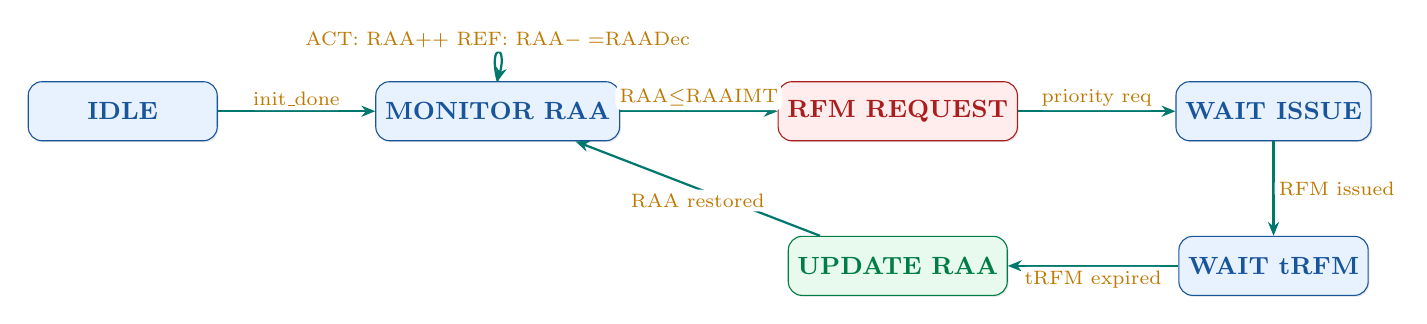
\begin{tikzpicture}[node distance=0.7cm and 2.2cm,>=Stealth]
  \node[fsm](MI)   {IDLE};
  \node[fsm,right=2cm of MI](MON)  {MONITOR RAA};
  \node[fsmred,right=2cm of MON](MRQ){RFM REQUEST};
  \node[fsm,right=2cm of MRQ](MIS) {WAIT ISSUE};
  \node[fsm,below=1.2cm of MIS](MT){WAIT tRFM};
  \node[fsmgreen,below=1.2cm of MRQ](MD){UPDATE RAA};

  \draw[arr](MI)   -- node[lbl,above]{init\_done} (MON);
  \draw[arr](MON)  -- node[lbl,above]{RAA$\leq$RAAIMT} (MRQ);
  \draw[arr](MON.north) to[loop above] node[lbl]{ACT: RAA++  REF: RAA$-=$RAADec}(MON.north);
  \draw[arr](MRQ)  -- node[lbl,above]{priority req} (MIS);
  \draw[arr](MIS)  -- node[lbl,right]{RFM issued} (MT);
  \draw[arr](MT)   -- node[lbl,below]{tRFM expired} (MD);
  \draw[arr](MD)   -- node[lbl,below]{RAA restored} (MON);
\end{tikzpicture}
\end{center}

\textbf{RAA Logic:}
$\text{RAA}[b] \mathrel{+}= 1$ on every ACT to bank $b$; \quad
$\text{RAA}[b] \mathrel{-}= \text{RAADec}$ on every REF to bank $b$. \\
When $\text{RAA}[b] \leq \text{RAAIMT}$: assert RFM request (priority above ZQcal, below refresh override).

\subsection{6d — Power Management FSM}

\begin{center}
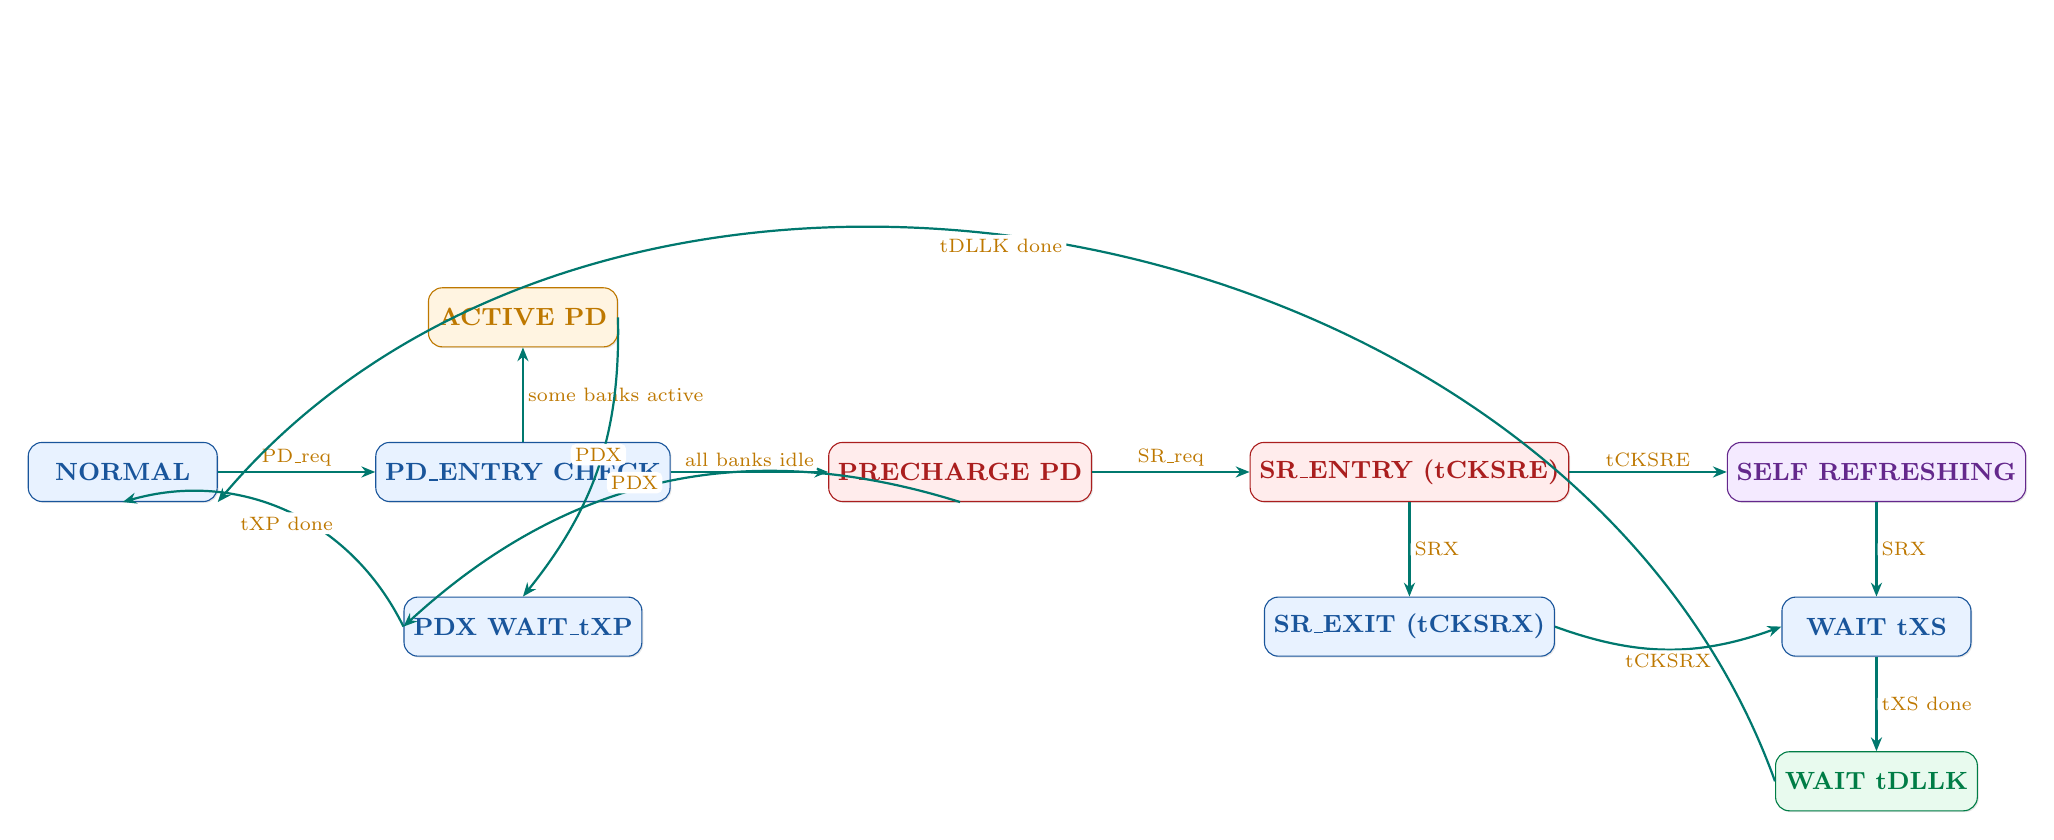
\begin{tikzpicture}[node distance=0.9cm and 1.8cm,>=Stealth]
  \node[fsm](NM)     {NORMAL};
  \node[fsm,right=2cm of NM](PDC)   {PD\_ENTRY CHECK};
  \node[fsmred,right=2cm of PDC](PDP){PRECHARGE PD};
  \node[fsmamber,above=1.2cm of PDC](PAP){ACTIVE PD};
  \node[fsm,below=1.2cm of PDC](PDX2){PDX WAIT\_tXP};
  \node[fsmred,right=2cm of PDP](SRE2){SR\_ENTRY (tCKSRE)};
  \node[fsmpurple,right=2cm of SRE2](SRF){SELF REFRESHING};
  \node[fsm,below=1.2cm of SRE2](SRX2){SR\_EXIT (tCKSRX)};
  \node[fsm,below=1.2cm of SRF](TXS2){WAIT tXS};
  \node[fsmgreen,below=1.2cm of TXS2](TDLL){WAIT tDLLK};

  \draw[arr](NM) -- node[lbl,above]{PD\_req} (PDC);
  \draw[arr](PDC) -- node[lbl,above]{all banks idle} (PDP);
  \draw[arr](PDC) -- node[lbl,right]{some banks active} (PAP);
  \draw[arr](PDP.south) to[bend right=30] node[lbl,left]{PDX} (PDX2.west);
  \draw[arr](PAP.east)  to[bend left=20]  node[lbl,above]{PDX} (PDX2.north);
  \draw[arr](PDX2.west) to[bend right=40] node[lbl,below]{tXP done} (NM.south);

  \draw[arr](PDP.east) -- node[lbl,above]{SR\_req} (SRE2.west);
  \draw[arr](SRE2) -- node[lbl,above]{tCKSRE} (SRF);
  \draw[arr](SRF.south) -- node[lbl,right]{SRX} (TXS2.north);
  \draw[arr](SRE2.south) -- node[lbl,right]{SRX} (SRX2.north);
  \draw[arr](SRX2.east) to[bend right=20] node[lbl,below]{tCKSRX} (TXS2.west);
  \draw[arr](TXS2) -- node[lbl,right]{tXS done} (TDLL);
  \draw[arr](TDLL.west) to[bend right=60] node[lbl,left]{tDLLK done} (NM.south east);
\end{tikzpicture}
\end{center}

%% ════════════════════════════════════════════════════════════
\section{Write Data Path}

\begin{longtable}{L{3.5cm} L{10.9cm}}
\toprule
\textbf{Sub-Block} & \textbf{Description} \\
\midrule
\endfirsthead\toprule\textbf{Sub-Block}&\textbf{Description}\\\midrule\endhead\bottomrule\endfoot
\rowcolor{rowblue}
Write Data Buffer     & Burst-aligned (BL16) FIFO storing data from CIF Write Cmd Pool. Dequeues when DFI write slot is confirmed by Scheduler. \\
DM/ECC Generator      & Computes per-byte Data Mask and inline ECC. Generates Write CRC (DDR5 §4.37) using CRC-8 polynomial over DQ+DM bits. \\
\rowcolor{rowblue}
WL Align              & Inserts programmable pipeline delay = CWL to align DQS preamble to DFI \texttt{dfi\_wrdata\_en}. \\
DFI Write Timing      & Drives \texttt{dfi\_wrdata}, \texttt{dfi\_wrdata\_mask}, \texttt{dfi\_wrdata\_cs\_n}, \texttt{dfi\_parity\_in}. Preamble per MR8 (2tCK default). ODT timing via tODTon/tODToff. \\
\rowcolor{rowblue}
Write CRC Error FSM   & States: \st{NORMAL}$\to$\st{CRC\_ERROR}$\to$\st{RETRY\_WR}$\to$\st{AUTO\_DISABLE}. Error detected via \texttt{dfi\_alert\_n}. Retry up to \textit{n} times (MR51/52); auto-disable CRC if threshold exceeded. \\
\end{longtable}

%% ════════════════════════════════════════════════════════════
\section{Read Data Path}

\begin{longtable}{L{3.5cm} L{10.9cm}}
\toprule
\textbf{Sub-Block} & \textbf{Description} \\
\midrule
\endfirsthead\toprule\textbf{Sub-Block}&\textbf{Description}\\\midrule\endhead\bottomrule\endfoot
\rowcolor{rowblue}
Read Latency Counter  & Per-outstanding-read counter. Tracks CL + read preamble cycles from RD command to expected data arrival from DFI. \\
Read Data FIFO        & Captures \texttt{dfi\_rddata} when \texttt{dfi\_rddata\_valid} asserted. Re-aligns burst-per-read. Feeds CIF Reorder Buffer. \\
\rowcolor{rowblue}
ECC/CRC Checker       & Verifies Read CRC (§4.37.7). On CRC error: flags to CIF error register; optionally triggers read retry. \\
ECS FSM               & States: \st{IDLE}$\to$\st{ECS\_ACTIVE}$\to$\st{WAIT\_tECS}$\to$\st{IDLE}. Triggered by MR14 (auto-ECS) or host MPC request. DRAM scrubs ECC during tECS window ($\leq$ tRFC1). \\
\end{longtable}

%% ════════════════════════════════════════════════════════════
\section{DFI 5.2 Interface Summary}

\begin{longtable}{L{4.5cm} L{2cm} L{8cm}}
\toprule
\textbf{Signal} & \textbf{Dir} & \textbf{Description} \\
\midrule
\endfirsthead\toprule\textbf{Signal}&\textbf{Dir}&\textbf{Description}\\\midrule\endhead\bottomrule\endfoot
\rowcolor{rowblue}
\sym{dfi\_address[13:0]}  & MC$\to$PHY & CA bus (2-cycle for DDR5 ACT) \\
\sym{dfi\_cs\_n[1:0]}     & MC$\to$PHY & Chip select (2 ranks) \\
\rowcolor{rowblue}
\sym{dfi\_cke[1:0]}       & MC$\to$PHY & Clock Enable per rank \\
\sym{dfi\_odt[1:0]}       & MC$\to$PHY & On-Die Termination control \\
\rowcolor{rowblue}
\sym{dfi\_reset\_n}       & MC$\to$PHY & DRAM RESET\_n \\
\sym{dfi\_wrdata[127:0]}  & MC$\to$PHY & Write data (BL16$\times$DQ8) \\
\rowcolor{rowblue}
\sym{dfi\_wrdata\_mask[15:0]} & MC$\to$PHY & Write data mask per byte \\
\sym{dfi\_wrdata\_en}     & MC$\to$PHY & Write data enable strobe \\
\rowcolor{rowblue}
\sym{dfi\_rddata[127:0]}  & PHY$\to$MC & Captured read data \\
\sym{dfi\_rddata\_valid}  & PHY$\to$MC & Read data valid flag \\
\rowcolor{rowblue}
\sym{dfi\_rddata\_dnv}    & PHY$\to$MC & Data-not-valid (error) \\
\sym{dfi\_alert\_n}       & PHY$\to$MC & DRAM alert (CRC error, parity) \\
\rowcolor{rowblue}
\sym{dfi\_ctrlupd\_req}   & MC$\to$PHY & Controller requests PHY update \\
\sym{dfi\_ctrlupd\_ack}   & PHY$\to$MC & PHY acknowledges update \\
\rowcolor{rowblue}
\sym{dfi\_phyupd\_req}    & PHY$\to$MC & PHY requests MC pause \\
\sym{dfi\_phyupd\_ack}    & MC$\to$PHY & MC acknowledges pause \\
\rowcolor{rowblue}
\sym{dfi\_parity\_in}     & MC$\to$PHY & CA parity (DDR5) \\
\sym{dfi\_wrdata\_cs\_n}  & MC$\to$PHY & Write CS\_n (DDR5 per-DRAM) \\
\end{longtable}

\begin{notebox}
\textbf{DFI timing:} \texttt{dfi\_wrdata\_en} must be asserted \texttt{tphy\_wrlat} cycles before write data.
\texttt{dfi\_rddata\_valid} arrives \texttt{tphy\_rdlat} cycles after the RD command is issued.
Both \texttt{tphy\_wrlat} and \texttt{tphy\_rdlat} are PHY-specific and communicated to the MC via DFI training.
\end{notebox}

%% ════════════════════════════════════════════════════════════
\section{FSM Summary Table}

\begin{longtable}{L{4cm} C{1.6cm} C{2cm} L{6.8cm}}
\toprule
\textbf{FSM} & \textbf{States} & \textbf{Instances} & \textbf{Notes} \\
\midrule
\endfirsthead\toprule\textbf{FSM}&\textbf{States}&\textbf{Instances}&\textbf{Notes}\\\midrule\endhead\bottomrule\endfoot
\rowcolor{rowblue}
Init FSM                    & 16 & 1  & Longest; spans RESET\_n to training complete \\
Bank State Machine (BSM)    & 11 & 16 & One per bank; $16\times11=176$ state bits \\
\rowcolor{rowblue}
DDR Cmd Scheduler           & 6  & 1  & Arbitrates all command types \\
Refresh Scheduler           & 6  & 1  & REFab/REFsb + FGR modes \\
\rowcolor{rowblue}
ZQcal FSM                   & 6  & 1  & MPC ZQCAL Start/Latch flow \\
RFM FSM                     & 5  & 1  & Per-bank RAA tracking \\
\rowcolor{rowblue}
Power Management FSM        & 10 & 1  & PD (Pre/Act) + SR + MPSM \\
Write CRC Error FSM         & 4  & 1  & Retry/auto-disable on dfi\_alert\_n \\
\rowcolor{rowblue}
ECS FSM                     & 4  & 1  & DDR5 inline ECC scrub window \\
\midrule
\rowcolor{lightgray}
\textbf{Total} & \textbf{$\approx$68} & \textbf{23} & \\
\end{longtable}

%% ════════════════════════════════════════════════════════════
\section{Timing Reference: Key Command Delays}

All values at @200\,MHz (tCK=5\,ns, CL=3, CWL=1, BL/2=8) and @100\,MHz (tCK=10\,ns).

\begin{longtable}{L{4.2cm} L{5.5cm} C{2cm} C{2cm}}
\toprule
\textbf{Command Sequence} & \textbf{Formula} & \textbf{@200\,MHz} & \textbf{@100\,MHz} \\
\midrule
\endfirsthead\toprule\textbf{Sequence}&\textbf{Formula}&\textbf{@200}&\textbf{@100}\\\midrule\endhead\bottomrule\endfoot
\rowcolor{rowblue}
ACT $\to$ RD/WR (same bank)    & tRCD                                & 4           & 4 \\
ACT $\to$ PRE (same bank, min) & tRAS                                & 7           & 4 \\
\rowcolor{rowblue}
PRE $\to$ ACT (same bank)      & tRP                                 & 4           & 4 \\
ACT $\to$ ACT (same bank)      & tRC = tRAS+tRP                      & 11          & 8 \\
\rowcolor{rowblue}
ACT $\to$ ACT (same BG)        & tRRD\_L                             & 4           & 4 \\
ACT $\to$ ACT (diff BG)        & tRRD\_S                             & 2           & 2 \\
\rowcolor{rowblue}
RD $\to$ RD (same BG)          & tCCD\_L                             & 8           & 8 \\
RD $\to$ RD (diff BG)          & tCCD\_S = BL/2                      & 8           & 8 \\
\rowcolor{rowblue}
WR $\to$ WR (same BG)          & tCCD\_L                             & 8           & 8 \\
WR $\to$ WR (diff BG)          & tCCD\_S = BL/2                      & 8           & 8 \\
\rowcolor{rowblue}
RD $\to$ WR (any)              & CL$-$CWL+BL/2+2+tWPRE              & 14          & 14 \\
WR $\to$ RD (same BG)          & CWL+BL/2+tWTR\_L                    & 13          & 13 \\
\rowcolor{rowblue}
WR $\to$ RD (diff BG)          & CWL+BL/2+tWTR\_S                    & 11          & 11 \\
RD $\to$ PRE (same bank)       & tRTP                                & 4           & 4 \\
\rowcolor{rowblue}
WR $\to$ PRE (same bank)       & CWL+BL/2+tWR                       & 15          & 12 \\
WRA $\to$ ACT (same bank)      & CWL+BL/2+tWR+tRP                   & 19          & 16 \\
\rowcolor{rowblue}
RDA $\to$ ACT (same bank)      & tRTP+tRP                            & 8           & 8 \\
REF $\to$ any                  & tRFC1                               & 39          & 20 \\
\rowcolor{rowblue}
SRX $\to$ ACT                  & tXS = tRFC1+10ns                    & 41          & 21 \\
PDX $\to$ any                  & tXP                                 & 5           & 5 \\
\rowcolor{rowblue}
MRW $\to$ MRW                  & tMRD                                & 16          & 16 \\
ZQcal start $\to$ latch        & tZQCAL = 1\,µs                      & 200         & 100 \\
\rowcolor{rowblue}
ZQCAL latch $\to$ next cmd     & tZQLAT                              & 30          & 30 \\
4 ACT window constraint        & tFAW                                & 2           & 2 \\
\bottomrule
\end{longtable}

%% ════════════════════════════════════════════════════════════
\section{Sub-Block Hierarchy}

\begin{center}
\begin{tikzpicture}[
  level 1/.style={sibling distance=4.8cm, level distance=1.4cm},
  level 2/.style={sibling distance=2.2cm, level distance=1.3cm},
  level 3/.style={sibling distance=1.8cm, level distance=1.2cm},
  every node/.style={draw=ddrblue,rounded corners=3pt,fill=rowblue,
                     font=\scriptsize\bfseries,text=ddrblue,
                     inner sep=3pt,minimum height=0.5cm},
  edge from parent/.style={draw=ddrteal,thick,-{Stealth[length=4pt]}}
]
\node {MC Core}
  child { node {Config Registers} }
  child { node {Init FSM}
    child { node {DLL Reset Seq} }
    child { node {ZQcal Init} }
    child { node {MRW Burst} }
  }
  child { node {Bank FSMs (×16)}
    child { node {Per-bank Timers} }
    child { node {State Register} }
  }
  child { node {Timing Control}
    child { node {Cross-BG Checker} }
    child { node {tFAW Window} }
  }
  child { node {Cmd Scheduler}
    child { node {Arbiter} }
    child { node {Page Policy} }
  }
  child { node {Maintenance Engine}
    child { node {Refresh FSM} }
    child { node {ZQcal FSM} }
    child { node {RFM FSM} }
    child { node {Power Mgmt FSM} }
  }
  child { node {Data Paths}
    child { node {Write Path} }
    child { node {Read Path} }
  };
\end{tikzpicture}
\end{center}

%% ════════════════════════════════════════════════════════════
\section{DDR5-Specific Additions vs DDR4}

\begin{longtable}{L{3.2cm} L{4.5cm} L{7cm}}
\toprule
\textbf{Feature} & \textbf{DDR4} & \textbf{DDR5 (MC Core Impact)} \\
\midrule
\endfirsthead\toprule\textbf{Feature}&\textbf{DDR4}&\textbf{DDR5}\\\midrule\endhead\bottomrule\endfoot
\rowcolor{rowblue}
REFsb (Same-Bank Refresh) & Not supported & Refresh Scheduler adds REFsb path; per-bank tRFCsb timer added to BSM \\
RFM (Rowhammer Mgmt) & Not supported & Full RFM FSM required; per-bank RAA counters; RAAIMT/RAAMMT Config Regs \\
\rowcolor{rowblue}
BL & BL8 (BL/2=4) & BL16 (BL/2=8); all timing formulae scale. RTW, WTR, WR-to-PRE all longer. \\
ACT command width & 1 cycle & 2-cycle CA encoding; Init FSM and Scheduler must drive CA on two consecutive rising edges \\
\rowcolor{rowblue}
ZQ mechanism & ZQCL/ZQCS commands & MPC ZQCAL Start+Latch; Init FSM restructured; ZQcal FSM uses MPC wrapper \\
tRFC1 (8\,Gb) & 350\,ns & 195\,ns; shorter refresh penalty; more scheduling headroom \\
\rowcolor{rowblue}
tREFI & 7.8\,µs & 3.9\,µs; double refresh rate; Refresh FSM budget counter halved \\
CWL definition & Separate table & CWL = CL$-$2; simpler Config Reg; Scheduler RTW formula simplified \\
\rowcolor{rowblue}
tMOD & 24\,nCK required & Replaced by tMRD only (16\,nCK); no separate tMOD path in Scheduler \\
ECS & Not supported & ECS FSM added in Read Data Path; hooks into tRFC window \\
\rowcolor{rowblue}
Write CRC & Optional (MR5) & Mandatory architecture support; dfi\_alert\_n monitoring; retry FSM required \\
PDA Enumerate & Basic PDA & Enhanced per-DRAM addressing; Init FSM extended sequence \\
\end{longtable}

%% ════════════════════════════════════════════════════════════
\vfill
\begin{center}
\small\textcolor{gray}{%
RMC MC Core Technical Specification ---
Memory Controller Capstone Project\\
JEDEC JESD79-5 (DDR5) / DFI 5.2 / AXI4
}
\end{center}

\end{document}
